% docs/texte/20_core/antennas.tex -- chapter "Antennas" (Interferosim)
% Version: 0.3.0 (2026-10-12) -- implementation (interferosim 0.3.0), beam figure
%   0.2.0: antenna types and proposals
%   0.1.0: placeholder
% ================================================================
\index{antenna types}

All antennas derive from the abstract class \texttt{Antenna} (gain,
effective area, half-power beam width, beam pattern); the parameters are
read from \texttt{configs/antennas/} (chapter~\ref{ch:data-formats}).
The relations between gain, effective area and beam width are given in
chapter \enquote{Radio Astronomical Fundamentals}.

\section{Types of the first version}

\begin{center}
\begin{tabular}{@{}l>{\raggedright\arraybackslash}p{5.0cm}>{\raggedright\arraybackslash}p{5.6cm}@{}}
\toprule
Type & Parameters & Use in the project \\
\midrule
Horn & gain (15\,dBi) & two-horn test with the Sun (notebook~B) \\
Parabolic dish & diameter, aperture efficiency, beam factor
  (3\,m, 0.60, 1.20) & mapping, long baseline (notebook~A) \\
Yagi & number of elements, boom length, gain, design frequency;
  linear polarisation & low-cost station antenna \\
\bottomrule
\end{tabular}
\end{center}

\section{Implementation}
\label{sec:antennas-impl}

The module \texttt{interferosim.instrument.antennas} implements the three
types as subclasses of \texttt{Antenna} (Fig.~\ref{fig:uml-model}).
\texttt{Antenna.from\_toml()} reads a file of \texttt{configs/antennas/};
the key \texttt{type} selects the class. All methods take the frequency
as argument (default: HI line).
\begin{itemize}
  \item \texttt{gain\_dbi(f)}, \texttt{effective\_area(f)} with
        $A_\mathrm{eff} = G\lambda^2/4\pi$, \texttt{hpbw\_deg(f)},
        \texttt{beam(theta\_deg, f)} (normalised power pattern, 1 on the
        axis) and \texttt{jy\_to\_k(f)} $= A_\mathrm{eff}/2k$.
  \item \textbf{Horn} and \textbf{Yagi} are defined by their gain. The
        main lobe is a rotationally symmetric Gaussian with
        $\Omega_A = 1.133\,\theta_\mathrm{HPBW}^2 = 4\pi/G$, i.\,e.\
        \begin{equation}
          \theta_\mathrm{HPBW} = \sqrt{\frac{4\pi}{1.133\,G}}
        \end{equation}
        (notebook~B). The gain of the horn is frequency independent; with
        the optional key \texttt{design\_freq\_hz} it is treated as a fixed
        aperture ($G\propto f^2$). The Yagi gain is valid near its design
        frequency. The values in \texttt{yagi.toml} are typical example
        values (13 elements, boom $0.85\,\mathrm{m}\approx 4\lambda$,
        $15\,\mathrm{dBi}$) until the data of the actual antenna are known.
  \item The \textbf{parabolic dish} follows \texttt{aas6sim}:
        $A_\mathrm{eff} = \eta\,\pi D^2/4$,
        $\theta_\mathrm{HPBW} = k\lambda/D$ ($k = 1.2$ for tapered
        illumination). Its beam is the Airy pattern of the uniformly
        illuminated aperture with the same HPBW,
        $d_\mathrm{eff} = 1.02\,D/k$:
        \begin{equation}
          P(\theta) = \left[\frac{2J_1(x)}{x}\right]^2,\qquad
          x = \frac{\pi d_\mathrm{eff}\sin\theta}{\lambda}.
        \end{equation}
        \texttt{otf(u, f)} is the transfer function of the filled circular
        aperture with the cut-off $u_\mathrm{cut} = d_\mathrm{eff}/\lambda$
        (\texttt{u\_cut\_eff}); $u_\mathrm{max} = D/\lambda$ would make the
        beam too narrow.
\end{itemize}

\begin{center}
\begin{tabular}{@{}lrrrrr@{}}
\toprule
Antenna & $f$ [MHz] & $G$ [dBi] & $A_\mathrm{eff}$ [m$^2$] & HPBW [$^\circ$] & SEFD$^*$ [Jy] \\
\midrule
Dish 3\,m  & 1420.406 & 30.78 & 4.241 &  4.84 & 78\,129 \\
           & 1665.402 & 32.16 & 4.241 &  4.13 & 78\,129 \\
Horn 15\,dBi & 1420.406 & 15.00 & 0.112 & 33.93 & 2\,955\,887 \\
           & 1665.402 & 15.00 & 0.082 & 33.93 & 4\,063\,508 \\
Yagi 13 el. & 1420.406 & 15.00 & 0.112 & 33.93 & 2\,955\,887 \\
\bottomrule
\multicolumn{6}{@{}l}{\footnotesize $^*$ with the B210, $T_\mathrm{sys} = 120\,\mathrm{K}$ (chapter~\ref{ch:receiver})}
\end{tabular}
\end{center}

\begin{figure}[htbp]
  \centering
  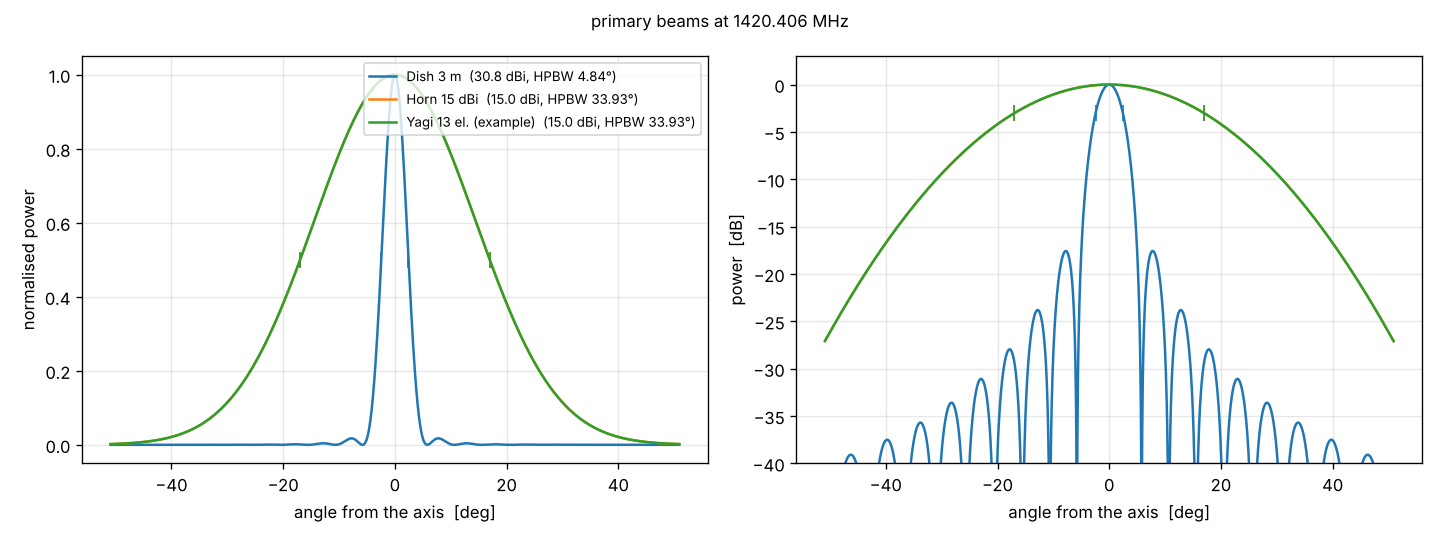
\includegraphics[width=\textwidth]{images/instrument_beams.png}
  \caption{Primary beams at $1420\,\mathrm{MHz}$ (\texttt{plot\_beams()}),
           linear and in dB; the bars mark the HPBW. Horn and Yagi
           coincide because both have $15\,\mathrm{dBi}$.}
  \label{fig:beams}
\end{figure}

\section{Proposals for further types}

\begin{center}
\begin{tabular}{@{}l>{\raggedright\arraybackslash}p{5.4cm}>{\raggedright\arraybackslash}p{5.2cm}@{}}
\toprule
Type & Properties & Why for Interferosim \\
\midrule
Axial-mode helix & circular polarisation, gain set by the number of
  turns, broader band than a Yagi & OH masers are often circularly
  polarised; Zeeman splitting (later extension) needs the circular
  components \\
Log-periodic dipole array (LPDA) & very broadband, moderate gain &
  one antenna for HI (1420\,MHz) and all four OH lines
  (1612--1720\,MHz) \\
Dipole (reference) & about 2.15\,dBi, very wide beam & reference
  antenna, Sun observations without tracking \\
Patch / patch array & flat, reproducible, gain grows with the number of
  patches & compact arrays of many elements for uv-coverage
  experiments \\
\bottomrule
\end{tabular}
\end{center}

Recommendation: helix and LPDA as the next two types -- the helix for the
polarisation of the OH lines, the LPDA for the frequency range of the
whole project. Further types need only a subclass of \texttt{Antenna}
and a configuration file.
